\documentclass{report}
\usepackage[T1]{fontenc} % Fontes T1
\usepackage[utf8]{inputenc} % Input UTF8
\usepackage[backend=biber, style=ieee]{biblatex} % para usar bibliografia
\usepackage{csquotes}
\usepackage[portuguese]{babel} %Usar língua portuguesa
\usepackage{blindtext} % Gerar texto automaticamente
\usepackage[printonlyused]{acronym}
\usepackage{hyperref} % para autoref
\usepackage{graphicx}
\usepackage{graphicx}
\usepackage{indentfirst}
\usepackage{placeins}
\usepackage{xfrac}
\usepackage{pgf-pie}


\bibliography{bibliografia}



\begin{document}
\def\titulo{\textbf{\Huge{Atletismo}}}
\def\data{\today}
\def\autores{Ana Monteiro, Bruno Lemos}
\def\autorescontactos{(98314) anamiguel24@ua.pt, (98221) blemos@ua.pt}
\def\departamento{\ac{DETI}}
\def\empresa{Universidade de Aveiro \\ Mestrado Integrado em Engenharia de Computadores e Telemática}
\def\logotipo{ua.pdf}

\begin{titlepage}

\begin{center}
%
\vspace*{50mm}
%
{\Huge \titulo}\\ 
%
\vspace{10mm}
%
{\Large \empresa}\\
%
\vspace{10mm}
%
{\LARGE \autores}\\ 
%
\vspace{30mm}
%
\begin{figure}[h]
\center
\includegraphics{\logotipo}
\end{figure}
%
\vspace{30mm}
\end{center}
%
\begin{flushright}
\end{flushright}
\end{titlepage}

%pagina de titulo%
\title{%
{\Huge\textbf{\titulo}}\\
{\Large \departamento\\ \empresa}
}
%
\author{%
    \autores \\
    \autorescontactos
}
%
\date{\data}
%
\maketitle

\pagenumbering{roman}

%resumo
\begin{abstract}

O atletismo faz parte da vida do ser humano, já desde a pré-história os nossos antepassados viam-se obrigados a correr para fugir dos predadores, a lanchar para caçarem os animais, ou simplesmente na marcha para se locomoverem. No entanto, com a evolução da espécie, o atletismo não ficando para trás acompanhou a evolução sofrendo várias modificações ao longo dos tempos, nomeadamente nos equipamentos utilizados.\par
Na atualidade existem várias disciplinas que fazem parte da modalidade do atletismo. As mais notórias são as corridas os saltos e os lançamentos e são estas mesmas que vão ser abordadas no trabalho. As corridas dividem-se em três estilos: velocidade, meio-fundo e fundo. Nos saltos encontramos 2 tipos: saltos horizontais e saltos verticais. Por fim os lançamentos dividem-se em quatro: lançamento do disco, lançamento do martelo, lançamento do peso e lançamento do dardo. \par
Na rotina diária de um atleta são vários os fatores influenciadores da prestação do mesmo no dia-a-dia, tais como o descanso, alimentação, tempos livres e de lazer, família entre outros. Destacando neste trabalho o sono que é dominado pelos dispositivos eletrónicos que imitem a chamada luz azul e a alimentação, que é um fator bastante importante, tal como dizia Hipócrates mais conhecido como o pai da medicina “Somos aquilo que comemos.”.\par
É importante dar valor às pessoas que merecem e que lutaram para alcançar um determinado objetivo. Assim há que destacar alguns recordes como o do Kevin Young em Barcelona no ano de 1992 e o do Leandro Ramos em Castellón no ano de 2019. É essencial ainda referir que o atleta nacional Francis Obikwelu nasceu na Nigéria mas apenas em Outubro de 2001 obteve nacionalidade portuguesa. Usain Bolt é um ex-velocista de origem jamaicana e é dos atletas mais famosos fora e dentro do atletismo. Mo Farah é um fundista britânico que possui todos os títulos possíveis da disciplina que pratica.

\end{abstract}

%\renewcommand{\abstractname}{Agradecimentos}
%\begin{abstract}
%Eventuais agradecimentos.
%Comentar bloco caso não existam agradecimentos a fazer.
%\end{abstract}

\tableofcontents
\listoftables     % descomentar se necessário
\listoffigures    % descomentar se necessário


%%%%%%%%%%%%%%%%%%%%%%%%%%%%%%%
\clearpage
\pagenumbering{arabic}

%%%%%%%%%%%%%%%%%%%%%%%%%%%%%%%%
\chapter{Introdução}
\label{chap.introducao}

O desporto faz, fez e fará parte da nossa vida. Praticamos desporto desde sempre. Embora, só um dos dois seja atleta federado na modalidade de atletismo, ambos nutrem por esta modalidade em particular, um interesse e uma paixão muito especial. Assim, na hora de escolher um tema para desenvolver, não foi difícil chegar a um consenso. Assim, neste trabalho iremos debruçar-mo-nos sobre o tema do atletismo, aprofundando conteúdos como a história, algumas disciplinas do atletismo, rotinas de um atleta e algumas curiosidades como recordes e lendas do atletismo. \par
Este documento está dividido em cinco capítulos.
Depois desta introdução, no \autoref{chap.História} é apresentada a história do atletismo focando a sua evolução. No \autoref{chap.Disciplinas} são apresentados várias provas existentes no atletismo, tais como: corridas (velocidade, meio-fundo e fundo), saltos (horizontais e verticais) e lançamentos (disco, martelo, peso e dardo). No \autoref{chap.Rotinasdiariasdeumatleta} são explicitado alguns hábitos diários que um atleta deve ter, tais como rotinas do sono e alimentares do atleta. No \autoref{chap.Curiosidades} são expostas algumas curiosidades como alguns recordes mundiais e celebridades impactantes do atletismo. Finalmente no \autoref{chap.Conclusões} é apresentada uma breve conclusão do tema.

         \FloatBarrier
            \begin{figure}[h]
            \center
            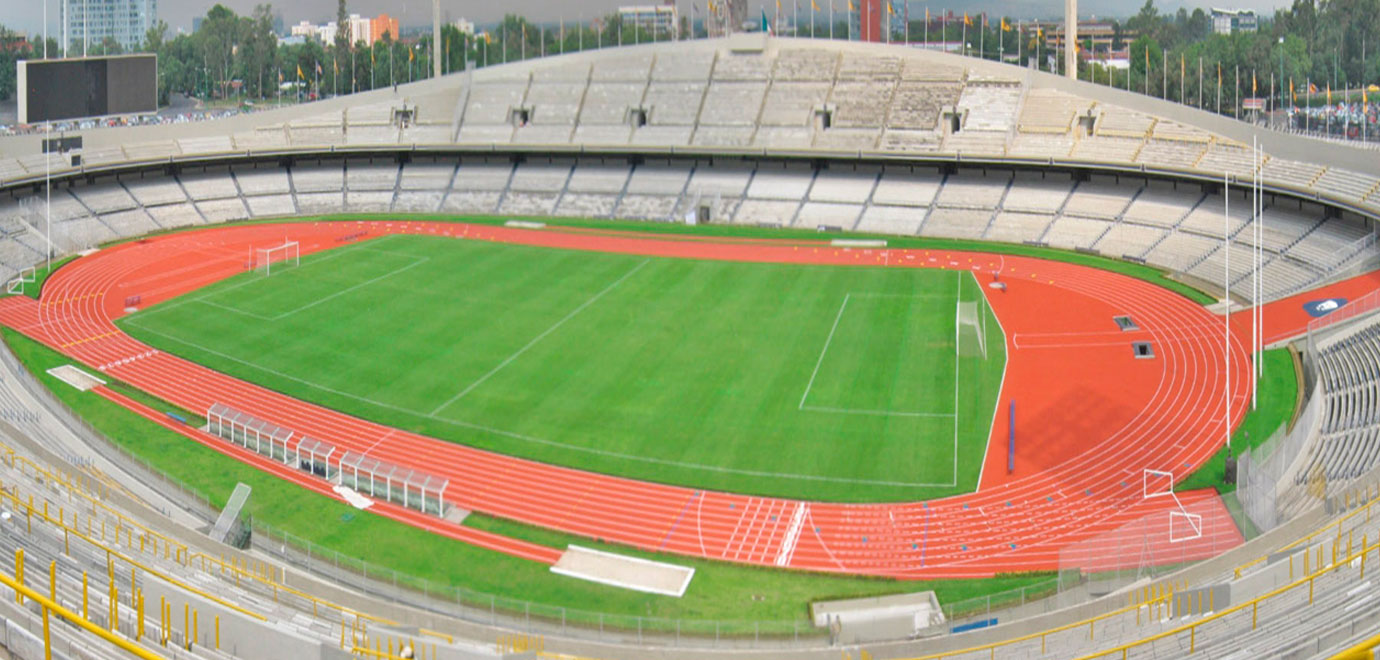
\includegraphics[scale=.20,angle=0]{pista.jpg}
            \caption{Pista de atletismo}
            \label{fig:pista.2}
            \end{figure}
            \FloatBarrier

\chapter{História}
\label{chap.História}
    
    \section{Origem do Atletismo }
    O atletismo é considerado o desporto mais antigo do mundo. Estima-se que este desporto surgiu à cerca de 4 mil anos atrás, no antigo Egito, onde eram realizadas diversas corridas entre elementos do género masculino. 
    Este desporto, na realidade, trata-se de uma mistura de vários desportos, englobando corridas, saltos e lançamentos que eram encarados como uma aprendizagem vital na caça e na guerra, nos tempos antigos. \par
    O ser humano já praticava algumas das modalidades do atletismo como forma de sobrevivência na pré-história. A caminhada, por exemplo, era utilizada para se locomover de um lugar para o outro. A corrida e os saltos, para escapar das presas dos animais carnívoros. Os lançamentos eram usados para se defenderem e matarem animais que serviam de alimento. Desta forma, os homens e as mulheres formam adquirindo habilidades que, mais tarde, foram aprimoradas e adaptadas para as competições de atletismo. Podemos dizer que os nossos antepassados eram por necessidade, grandes atletas. Só os mais fortes, os mais resistentes, os mais rápidos, ou seja, os mais ágeis é que sobreviviam nas melhores condições. \cite{origemdoatletismo}
   
    \section{Atletismo na atualidade}
    O Atletismo ao longo dos tempos tem vindo a evoluir de tal forma que os resultados têm sido melhorados e atingidos vários recordes. As condições dos equipamentos têm ajudado para a evolução deste desporto, tanto no âmbito de equipamentos pessoais, calçado e vestuário mais confortável e adequado, como nas instalações e condições de treino que se encontram ao dispôr da generalidade dos atletas como, por exemplo,  pistas de atletismo de tartan melhorado em relação às suas características e funcionalidades iniciais; blocos de partida anatomicamente mais adequados; condições climatéricas condicionadas no estádio; equipamentos de ginásio mais sofisticados e que proporcionam resultados mais rápidos, entre outras melhorias significativas fruto do investimento e da inovação existente. \par
    Uma das evoluções mais notórias são as tecnologias que foram acompanhando este desporto. Atualmente,  a cronometragem é feita através de sensores e cronómetros digitais, tudo com tecnologia muito mais avançada e sofisticada, do que era antigamente, permitindo uma fiabilidade dos resultados obtidos muito mais precisa.
    Uma das mudanças significativas e numa área totalmente diferente da abordada anteriormente, diz respeito à igualdade entre homens e mulheres no acesso a muitas das provas nesta modalidade.  A possibilidade das mulheres realizarem algumas provas nas disciplinas que lhes foram sendo vedadas, ao longo dos tempos, foi lenta e progressiva. Pode-se afirmar, que neste momento, as mulheres já podem realizar todas as provas que os homens realizam, sendo que os 50Km marcha foi uma das últimas provas a serem abertas ao setor feminino. \cite{origemdoatletismo}
    
    \hfill \newline
    \hfill \newline
    
     \FloatBarrier
            \begin{figure}[h]
            \center
            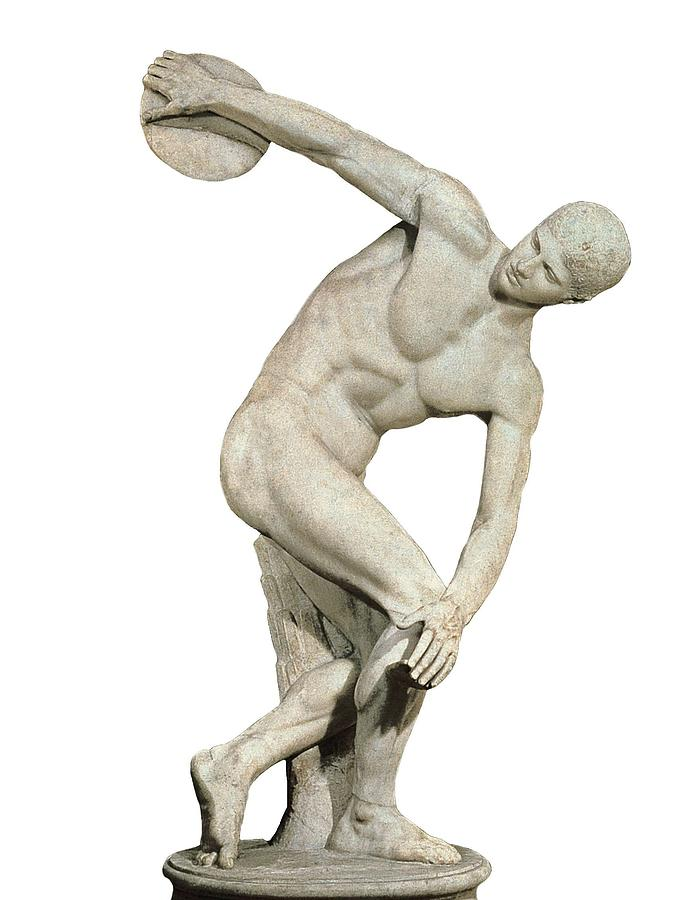
\includegraphics[scale=1,angle=0]{estatua.jpg}
            \caption{O Discóbolo (Diskobólos, lançador de disco) de Míron}
            \label{fig:blocos.2}
            \end{figure}
    \FloatBarrier

\chapter{Disciplinas}
\label{chap.Disciplinas}

    \section{Corridas}
        \subsection{Corridas de velocidade}
        As corridas de velocidade dividem-se em provas individuais que incluem corridas ao ar livre (100 metros, 200 metros, 400 metros, 100 metros barreiras para feminino e 110 metros barreiras para masculino e 400 metros barreiras) e corridas de pista coberta (60 metros, 400 metros, 60 metros barreiras) e provas em equipas que incluem as estafetas (4x100 metros e 4x400 metros). Nestas provas os atletas estão impedidos de ocupar um corredor da pista que não lhes foi destinada. Caso isso ocorra o atleta é automaticamente desclassificado. \par
        Este tipo de corrida é iniciado em blocos de partida, os procedimentos de partida são controlados por um juiz através de comando de voz pela seguinte ordem: aos seus lugares, em que os atletas se dirigem para os blocos e respetiva pista; prontos, em que os atletas se põem em posição para a partida; e um sinal sonoro que normalmente é um tiro em que os concorrentes iniciam a sua corrida.
        Durante a corrida os atletas devem passar por 4 fases essenciais, a partida, o alcance da velocidade, a manutenção da velocidade e a redução de velocidade.
        
         \FloatBarrier
            \begin{figure}[h]
            \center
            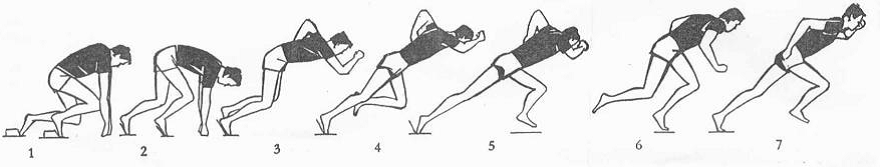
\includegraphics[scale=.3,angle=0]{velocidade.png}
            \caption{Saída de blocos em provas de velocidade}
            \label{fig:blocos.2}
            \end{figure}
          \FloatBarrier
    
            \subsubsection{Corridas ao ar livre}
            Na corrida ao ar livre de 100 metros os atletas correm sempre em linha reta, por outro lado na corrida de 200 metros e na de 400 metros os atletas percorrem curvas, tendo de gerir bem a capacidade de velocidade, de técnica e de gestão de esforço. Nas provas de barreiras as mulheres percorrem os 100 metros e os homens correm 110, no caso dos 400 metros ambos os sexos percorrem a mesma distância. Estas provas são caracterizadas por serem de um elevado grau de dificuldade. Caso os atletas derrubem uma barreira não são desclassificados, apenas é mau para a sua prestação pois perdem bastante tempo.
            \subsubsection{Corridas em pista coberta}
            Nas corridas de pista coberta de 60 metros os atletas correm em linha reta, na de 400 metros os atletas para completarem a prova têm de dar duas voltas completas à pista em que nos primeiros 150 metros os atletas correm em pistas individuais na marca dos 150 “vão à corda” e correm todos na pista um. Na prova de 60 metros barreiras os atletas têm de transpor barreiras que são postas na pista.
            \subsubsection{Estafetas - Prova coletiva}
            Na corrida de estafetas as equipas são constituídas por 4 elementos. Na prova de 4x100 metros cada atleta corre 100 metros e na prova 4x400 metros cada atleta corre 400 metros. Cada um corre um determinado percurso, tendo de passar ao seu colega de equipa o testemunho na zona de transmissão, tendo também de ser passado de mão para mão, caso contrário são desclassificados. \cite{velocidade}
            
    \hfill \newline
    \subsection{Corridas de meio-fundo}
    As corridas de meio fundo que existem no atletismo são os 800m, 1500m e 3000m ( em pista coberta ). Estas provas, mesmo não sendo essencialmente corridas tão rápidas como as de velocidade pura, são extremamente duras, porque é necessário na mesma a velocidade a par da resistência.  \par
    Nesta corrida os atletas têm de ter a capacidade de observar os outros atletas e avaliar todos os movimentos para possíveis mudanças de ritmo. A capacidade mental/psicológica também deve ser excelente para suportar com grande eficiência as adversidades que decorrem na prova.
    \begin{itemize}
        \item Nos 800m os atletas percorrem 2 voltas completas à pista. Após a partida os atletas correm em pistas individuais e só depois da primeira curva (primeiros 100m) os atletas "cortam à corda" e vão para a pista de dentro.
        \item Os 1500m são a principal prova do meio fundo e as principais características dos atletas são bastante semelhantes, com maior ênfase na resistência aeróbica e menor na velocidade, em termos puros. Para o atleta completar uma prova de 1500m o atleta tem de percorrer 3 voltas completas e \sfrac{3}{4} de uma volta.
    \end{itemize}
    
    As principais qualidades dos atletas fisicas dos atletas são a velocidade, resistência, boa e controlada respiração circulatória. Por outro lado também têm qualidades psicológicas: fibra, e muita força de vontade. \par
    Por estes motivos, os atletas que praticam meio fundo são os atletas mais completos, porque possuem todas as caracteristicas. \cite{corridameiofundo}
 
    \hfill \newline    
    \subsection{Corridas de fundo}
    As corridas de fundo são corridas de longas distâncias, são elas os 5000m, 10000m, meia maratona e maratona. A maratona é a prova mais popular das corridas de fundo. Enquanto que numa corrida de 100m é necessário uma grande potência muscular para atingir grandes velocidades, na corrida de fundo será necessário uma resistência muito maior que o habitual. Um atleta com muita velocidade pode ter sucesso nas corridas de velocidade, por outro lado falhar numa corrida de longa distância. \par
    \begin{itemize}
        \item A corrida de 5000m e 10000m são as únicas corridas de pista ao ar livre que são corridas de fundo. Este tipo de corrida necessita de um mínimo de velocidade, no entanto a resistência é o fator mais importante. As principais nações com melhores resultados nestas disciplinas são o Quénia e a Etiópia.
        \item A meia maratona e a maratona são as principais provas de fundo que são praticadas na estrada. Na maratona são corridos 42,195km, é das corridas mais longas do atletismo e das mais conhecidas. A maratona tem vários praticantes, tanto profissionais como amadores, sendo estes últimos em maior número.\cite{corridafundo}
    \end{itemize}
        
    \section{Saltos}
    Os saltos são uma modalidade do atletismo onde os atletas combinam velocidade, força e agilidade para executarem o salto mais longe possível a partir de um ponto pré-definido
    
        \subsection{Saltos horizontais}
        Existem dois tipos de saltos horizontais, comprimento e triplo salto. Em ambos os saltos existe corrida de balanço, tábua de chamada e uma área onde o atleta cai (caixa de areia).
            \subsubsection{Salto em comprimento}
            O salto em comprimento consiste em uma corrida de cerca de 30 metros ou mais,que também é conhecida como zona de balanço,depois é seguido de um \textit{setp} a partir da tábua até à caixa de areia. O saltador, depois da impulsão, lança as pernas para a frente para aterrar o mais longe possível na caixa de areia. Cada atleta tem três saltos após isso são escolhidos os oito melhores para mais três saltos, chamada a Final. \par
            Há três técnicas possíveis no salto em comprimento que se distinguem pelas
            acções que os atletas fazem durante a fase de voo.
            \begin{itemize}
                \item A técnica da extensão é normalmente utilizada por atletas mais fortes, de grande potência muscular e a maioria das vezes pelas mulheres. 
                \item A técnica da tesoura é utilizada por atletas que têm a velocidade como o ponto mais forte da sua prova.
                \item A técnica da passada é a menos complexa, por isso mesmo é utilizada na formação dos atletas mais jovens. Contudo existe.
            \end{itemize}
            
            \FloatBarrier
            \begin{figure}[h]
            \center
            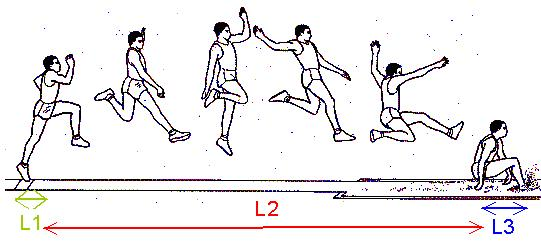
\includegraphics[scale=.45,angle=0]{saltocomprimento.JPG}
            \caption{Fases do salto em comprimento}
            \label{fig:saltocomprimento.2}
            \end{figure}
            \FloatBarrier
            
            
            \subsubsection{Triplo salto}
            O triplo salto é uma combinação de três saltos sucessivos que terminam na caixa de areia. A prova é iniciada com uma corrida de impulso e passa por 3 fases distintas: \textit{hop}, \textit{setp} e \textit{jump}.
            
            \begin{itemize}
            
            
            \item
            O \textit{hop} consiste no primeiro apoio do triplo salto que por norma é efetuado com a perna mais forte e é necessário a troca de pernas em fase de voo (movimento de tesoura).
            
            
            \item 
            O \textit{step} consiste no segundo contacto com o chão, onde o impacto é de grande intensidade. A perna de impulsão sofre uma pressão equivalente até 6 vezes o peso do atleta. A chamada para esta fase é efetuada através de um movimento brusco com a perna de modo que a velocidade não se reduza por completo. O movimento de braços é crucial para manter o equilíbrio através da rotação horizontal dos braços, mantendo a gravidade bem alinhada.
            
            
            
            \item 
            O \textit{jump} é geralmente realizado através da perna mais fraca, a perda de velocidade deve ser mínima de modo a aumentar esta fase do triplo salto. Esta fase pode ser facilmente comparada a fase final do comprimento ( finalização ) onde a correcção do equilíbrio é fundamental e é feita com braços nessa mesma fase de voo. \cite{salto}
            
            \end{itemize}
            
            \FloatBarrier
            \begin{figure}[h]
            \center
            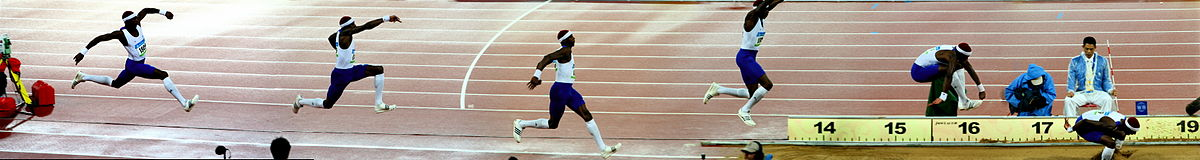
\includegraphics[scale=.25,angle=0]{triposaltoCOMPLETO.jpg}
            \caption{Fases do triplo salto}
            \label{fig:saltocomprimento.2}
            \end{figure}
            \FloatBarrier
    
    
    
    
    
    
    
        \subsection{Saltos verticais}
        Existem dois tipos de saltos verticais, salto com vara e salto em altura. Ambos os saltos implicam transpor uma fasquia que ]e colocada a uma altura predefinida pelos atletas mesmo antes da competição começar. Ao longo da prova a fasquia vai aumentando aos poucos de acordo com a passagem, válida ou não, dos atletas. 
            \subsubsection{Salto com vara}
            No salto com vara (Fibra de vidro) os atletas usam uma vara longa e flexível para alcançar a fasquia,barra horizontal, que ao longo da prova vai aumentando a sua altura. Essa progressão deve ser feita, no mínimo, de 5 em 5 centímetros. O atleta usa a vara, sobre o chão, para ganhar altura para passar a fasquia, caindo num colchão para evitar a lesão. Os atletas têm três tentativas para cada altura, ao fim da terceira falta o atleta está fora da prova. O salto com vara tem quatro fases principais:
            \begin{itemize}
                \item  Corrida de aproximação – O atleta deve efetuar uma corrida de balanço com bastante domínio dos movimentos para que não interfira nas fases seguintes.
                \item Encaixe – Nesta fase o objetivo do saltador é aumentar a sua energia cinética, resultante da velocidade atingida na fase posterior. No final desta fase a energia cinética do saltador começa a ser transferida para a vara, através do encaixe da vara no solo.
                \item Impulsão – Esta fase é a fase mais importante do salto com vara. Esta fase é responsável pela transferência da energia da corrida para só depois efetuar o salto com a seguinte sequência, pêndulo, a elevação e o giro.
                \item Elevação e giro – Assim que a vara recupera a sua forma natural , esta fase inicia-se. Primeiro elevam-se as pernas e depois os quadris ultrapassam a linha da vara e depois e é efetuado a recolha da vara do atleta.
                \cite{saltovara}
            \end{itemize}
           
            
            
            
            \FloatBarrier
            \begin{figure}[h]
            \center
            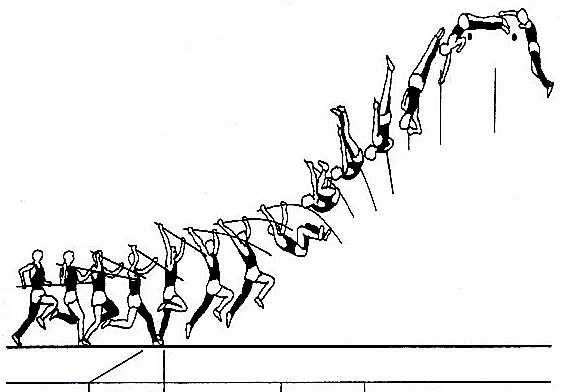
\includegraphics[scale=.4,angle=0]{saltocomvara.jpg}
            \caption{Salto com vara}
            \label{fig:vara.2}
            \end{figure}
            \FloatBarrier
            
            
            
            \subsubsection{Salto em altura}
            O salto em altura é considerado um salto vertical e  pode ser divido em 3 fases:  posição inicial, corrida e impulsão. 
            
             \FloatBarrier
            \begin{figure}[h]
            \center
            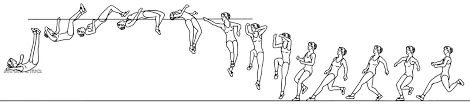
\includegraphics[scale=.42,angle=0]{saltoaltura.jpg}
            \caption{Salto em altura}
            \label{fig:saltoaltura.2}
            \end{figure}
            \FloatBarrier
            
            \begin{itemize}
                \item Posição Inicial 
                \par De forma geral o atleta coloca-se, no ponto inicial da corrida, com os dois pés unidos, braços soltos ao longo do resto do corpo e a observar/analisar a fasquia. Desta forma o atleta concentra-se para o salto.
                
                \item Corrida 
                \par A fase da corrida é das fases mais importantes para que as fases seguintes funcionem, deste modo a importância dada a esta fase da prova. A velocidade do atleta é fundamental mas na prova é necessário controlo para permitir ao atleta a melhor conversão do movimento ( do horizontal para o quase vertical ). É uma corrida em progressão, onde a velocidade máxima é atingida momentos antes do salto em si.  /par
                Podemos separa a corrida em duas partes:  inicial e final.
                
                \begin{enumerate}
                    \item A inicial, com velocidade progressiva, com o corpo mais solto e passadas um pouco mais abertas. O objetivo principal desta fase é adquirir velocidade inicial para, só depois, passar para a segunda fase.
                    \item A outra parte é a final, que se resume aos últimas três/cinco passadas, dependendo do atleta. Estas últimas passadas da corrida devem ser bastante mais rápidas que as passadas da fase inicial. Através disso, o corpo sofre uma ligeira inclinação para trás que altera o centro de gravidade, aproximando-o do chão. O pé de impulsão dista cerca de 70 cm da fasquia.
                \end{enumerate}
                
                \item Impulsão 
                \par Para efetuar esta fase da forma correta é necessário um bom aproveitamento da fase de corrida, por causa da velocidade.  Desta forma maximizamos a força da perna de impulsão e posteriormente o salto é maior. Caso a execução seja menos correta, em alguma das fases, retira quais quer possibilidades de resultar num bom salto.
                O impulso é dividido em duas fases distintas.
                \begin{enumerate}
                    \item O primeiro é movimento da perna livre que de certa forma tem como objetivo equilibrar o corpo e aliviar o peso do corpo.
                    \item A segunda é referente ao movimento da perna de impulsão, que aproveita a corrida para elevar o corpo para cima com toda a potência possível (força de impulsão + velocidade). Quanto ao movimento dos braços, em todo o movimento, devem equilibrar o corpo, tal como a perna livre.
                \end{enumerate}
                
            \end{itemize}
            \cite{salto}


               
    
    \section{Lançamentos}
    %FALAR SOBRE OS LANÇAMENTOS DE FORMA GERAL
    Existem lançamentos de quatro engenhos diferentes: disco, martelo, peso e dardo. O objetivo de qualquer um dos lançamentos é lançar o instrumento o mais longe possível, utilizando técnicas especificas. Todos estes tipos de lançamentos se dividem na categoria feminina e masculina, variando assim as características dos engenhos (peso, largura, espessura, etc…). O que pode variar também é o local onde é lançado o engenho, sendo que o lançamento de disco e do martelo é realizado na mesma secção e a dos restantes lançamentos em secções diferentes. \par
    Um lançamento é nulo quando:
    \begin{itemize}
        \item 
        o instrumento cair fora do sector destinado à queda do mesmo;
        \item
        o lançador pisa ou transpõe com qualquer parte do corpo as delimitações da zona de lançamento;
        \item
        o atleta sai da zona de lançamento antes de o engenho cair no solo;
        
    \end{itemize}
    
    
        \subsection{Lançamento do disco}
        O disco na categoria masculina pesa 2 Kilo, tem 22 centímetros de diâmetro e 45 milímetros de espessura, já o disco na categoria feminina pesa 1 Kilo, tem 18 centímetros de diâmetro e 38 milímetros de espessura.\par
        Procedimentos do lançamento:
        \begin{enumerate}
            \item O atleta deve executar o lançamento segurando o disco com o apoio dos dedos da mão e do antebraço;
            \item de seguida deve girar uma vez sobre o seu corpo;
            \item lançar o disco tentando que este alcance a maior distância possível.
        \end{enumerate} \cite{lancamentodisco}

    \hfill \newline
     \FloatBarrier
            \begin{figure}[h]
            \center
            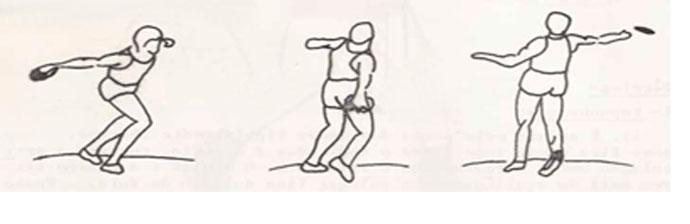
\includegraphics[scale=.4,angle=0]{disco.jpg}
            \caption{Lançamento do disco}
            \label{fig:disco.2}
            \end{figure}
            \FloatBarrier

   

    \subsection{Lançamento do martelo}
    O martelo é constituído por uma bola de ferro presa a uma alça por um arame metálico.
    O peso total do engenho na categoria masculina é 7,26 kilos e na categoria feminina é 4 kilos. \par
    O procedimento de lançamento divide-se em 3 etapas:
    \begin{enumerate}
        \item o lançador inicia o movimento virado de costas para a secção de lançamento, segurando a alça com as duas mãos e mantendo os pés imóveis;
        \item gira o martelo três ou quatro vezes para que este ganhe velocidade;
        \item por fim quando o martelo ganha velocidade suficiente, lança-o para a frente e para a cima.
    \end{enumerate} \cite{lancamentomartelo}
    
    \hfill \newline
     \FloatBarrier
            \begin{figure}[h]
            \center
            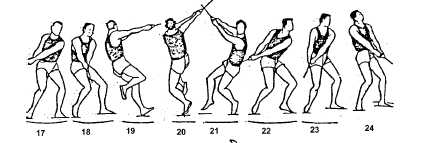
\includegraphics[scale=.5,angle=0]{martelo.png}
            \caption{Lançamento do martelo}
            \label{fig:martelo.2}
            \end{figure}
    \FloatBarrier

    \subsection{Lançamento do peso}
    O peso é constituído por ferro fundido e chumbo ou bronze.
    Na categoria masculina o instrumento pesa 7,26 kilos e tem o diâmetro de cerca de 12 centímetros, já na categoria feminina pesa 4 kilos e tem um diâmetro de 9 centímetro.\par
    Para fazer o lançamento é necessário seguir os seguintes passos:
    \begin{enumerate}
        \item o atleta está de costas para a secção de lançamento e coloca o engenho entre o pescoço e o ombro do atleta (utilizando um pó quando necessário para diminuir o atrito);
        \item o atleta gira sobre o seu próprio eixo para que o engenho adquira velocidade;
        \item por fim lança o engenho para a frente e para cima.
    \end{enumerate}
    \cite{lancamentodopesodardo}
    
    \hfill \newline
     \FloatBarrier
            \begin{figure}[h]
            \center
            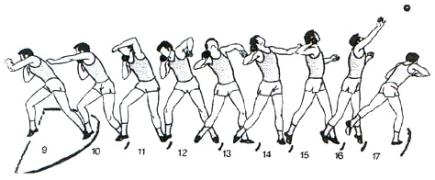
\includegraphics[scale=.5,angle=0]{peso.jpg}
            \caption{Lançamento do peso}
            \label{fig:peso.2}
            \end{figure}
    \FloatBarrier
    \hfill \newline

    \subsection{Lançamento do dardo}
    O engenho utilizado, dardo, é constituído por uma pega de corda a meio do engenho e por uma ponta de metal que é a primeira região a tocar no solo. Na categoria masculina o dardo possui um comprimento de 2,7 metros e pesa 0,8 kilos, no que toca à categoria feminina, o dardo possui 2,3 metros de comprimento e pesa 0,6 kilos. \par
    O lançamento é feito numa zona restrita, formada por um corredor de balanço de 4 metros de largura e um arco de um círculo que tem um raio de 8 metros e a zona de queda.\par 
    Para efetuar o lançamento há que seguir os seguintes passos: 
    \begin{enumerate}
        \item
        corrida de balanço;
        \item
        posição de lançamento;
        \item
        projeção do dardo; 
        \item
        recuperação do equilíbrio.
    \end{enumerate} \cite{lancamentodopesodardo}
    
     \FloatBarrier
            \begin{figure}[h]
            \center
            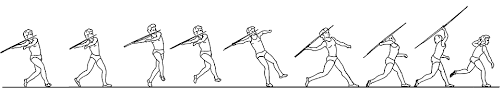
\includegraphics[scale=.55,angle=0]{dardo.png}
            \caption{Lançamento do dardo}
            \label{fig:dardo.2}
            \end{figure}
    \FloatBarrier
    
    \chapter{Rotinas diárias de um atleta}
    \label{chap.Rotinasdiariasdeumatleta}
    \section{Dia-a-dia do atleta}
    Do dia-a-dia de um atleta fazem parte um conjunto de atividades e comportamentos que muito influenciam o seu desempenho desportivo. Assim o atleta não deve descurar aspetos como o descanso, a alimentação, a higiene, os tempos livres, a família, os amigos, entre outros.\par
    \renewcommand{\theenumi}{\roman{enumi}}
    \begin{enumerate}
        \item Os atletas acordam muitas vezes cedo, e em parte dos dias aproveitam para treinar logo pela manhã. Benefícios de levantar cedo: primeiro o dia torna-se mais produtivo, aumenta a concentração, melhora o humor e diminui o stress.
        \item Ir para a cama cedo também é importante para o dia seguinte se tornar produtivo, devem ir dormir não antes das 23h e devem deixar de utilizar equipamentos eletrónicos 30 minutos antes da hora de sono.
        \item O descanso pós treino, principalmente os mais intensos e pós prova, também é importante para que os músculos tenham tempo de recuperar.
        \item Desfrutar dos tempos livres e ocupá-los com atividades de lazer é importante para a saúde mental do atleta.
        \item Um atleta deve comer várias vezes ao longo do dia. Os benefícios que traz para o atleta são os seguintes: 
        \begin{itemize}
            \item Evita que coma demais;
            \item mantem os níveis de glicerina constantes, ou seja, a taxa de açúcar no sangue mantem-se em níveis normais;
            \item acelera o metabolismo;
            \item a vontade de comer, ou sensação de fome diminui.
        \end{itemize}
        \item Um atleta não pode consumir substâncias psicoativas, como o álcool, tabaco, anfetaminas, cloridrato de cocaína, entre outras.
    \end{enumerate}
    
    No seguimento do trabalho irá ser aprofundados os temas do sono e da alimentação.


    \subsection{Importância do sono}
    O sono assume um papel fundamental na qualidade de vida de qualquer ser humano, sendo ainda mais relevante na vida de um atleta.
    Dormir o número de horas recomendáveis torna-se imprescindível para uma boa recuperação quer a nível físico, quer a nível psicológico do atleta.\par
    Além do cuidado de dormir o número de horas necessárias a um bom descanso o atleta deverá ter o cuidado de desligar atempadamente todos os aparelhos eletrónicos, nomeadamente a televisão e o telemóvel, pois a luz que emitem transmite ao cérebro a sensação de que está de dia, afetando assim, o relógio biológico e retardando a hora e sensação de sono. A luz azul diminui a qualidade do sono, pois anula duas vezes mais a produção de melatonina, hormona que regula o ciclo do sono e determina quando é hora de dormir e de acordar. Esta hormona é produzida no cérebro e a sua produção depende da luz emitida pelos equipamentos. Por outro lado, o conteúdo visto na tela também pode estimular o cérebro e retarda a vontade de dormir. \cite{sono}
    
    \subsection{Importância da alimentação}
    
    A alimentação, a par do sono, é outro fator fulcral, para que um atleta esteja em boa forma e tenha o rendimento e desempenho pretendido. \par
    A dieta alimentar de um atleta deve ser planeada consoante a modalidade praticada, os objetivos que se pretende alcançar e as características de cada atleta, ou seja, nem todos os atletas precisam da mesma dieta nem dos mesmos valores nutricionais. \par
    
    
    Os pontos essenciais para a dieta de qualquer atleta são:

    \renewcommand{\theenumi}{\alph {enumi}}
    \begin{enumerate} 
        \item hidratação constante;
        \item nunca ir de jejum para treinos;
        \item consumo moderado de alimentos possuidores de cafeína.
    \end{enumerate} 
    
 
    
    De uma alimentação equilibrada e nutritiva para atletas recomendam-se os seguintes alimentos:
    
    \renewcommand{\theenumi}{\alph {enumi}}
    \begin{enumerate}
        \item Banana – fonte de potássio, que ajuda na prevenção de cãibras;
        \item Aveia – fonte de carboidratos, que regula o açúcar no sangue e aperfeiçoa a saúde cardíaca;
        \item Batata-doce – fonte de potássio e de fibras com baixo teor em calorias;
        \item Nozes – fonte de proteína, ricos em gorduras boas, antioxidantes e vitamina E;
        \item Vegetais verdes – pobres em calorias, porém possuem bastantes minerais;
        \item Laranja – rica em vitamina C que funciona como antioxidante e ajuda os músculos doridos a recuperar mais rapidamente.
    \end{enumerate}
    
    A dieta deve ser programada tendo em conta a quantidade de calorias que o atleta gasta durante a atividade. Em média numa corrida de meia hora gasta-se 350 calorias. \par
    Do atletismo fazem parte várias disciplinas do grupo das corridas, dos saltos e dos lançamentos. Consoante a disciplina praticada, o treino realizado e provas disputadas são solicitados mais uns grupos musculares do que outros, são realizados esforços mais ou menos intensos daí a alimentação e os alimentos a escolher terem que variar. \par 
    Para além do referido no parágrafo anterior, há a referir outros fatores que interferem e fazem variar a quantidade de calorias gastas, como por exemplo, a idade do atleta, se o atleta está lesionado, o tempo de treino e a intensidade do mesmo. A acrescentar temos ainda a questão da temperatura, que em algumas situações e para algumas pessoas a sua importância passa despercebida. Quando está calor o nosso corpo tem de se esforçar mais, o que leva a um cansaço mais rápido, por outro lado, quando está frio o corpo é obrigado a fazer um esforço extra até atingir uma temperatura normal. Na generalidade treinar em épocas com temperaturas amenas permite ao atleta um treino com "aparente" menor cansaço físico e em boas condições, durante mais tempo permitindo uma melhor performance. \cite{alimentacao}
    \hfill \newline
    \hfill \newline
    \begin{figure}[h]
    
        \begin{center}
            \begin{tikzpicture}
                \pie [rotate = 180]
                {20/\ac{Fru} , 2/\ac{GO} , 18/\ac{LD} , 4/\ac{CPO} , 5/\ac{Leg} , 28/\ac{CT} , 23/\ac{Hort}}
            \end{tikzpicture}
            \caption{Alimentação de um atleta}
        \end{center}
    \end{figure}

    
    \chapter{Curiosidades}
    \label{chap.Curiosidades}
    \section{Alguns recordes}
    \subsection{Recordes nacionais}
    \begin{table}[h]
    \caption{Recordes Nacionais}
        \begin{tabular}{|c|c|c|c|c|}
            \hline
            Prova & Atleta & Marca & local & data  \\ \hline
            100m & Francis Obikwelu & 9.86s & Atenas & 22-08-2004 \\ \hline
            200m & Francis Obikwelu & 20.01s & Gotemburgo & 10-08-2006 \\ \hline
            400m & Vítor Ricardo Santos & 45.14s & Berlim & 10-08-2018 \\ \hline
            800m & Rui Silva & 1.44.91 & S. Sebastian & 20-08-2002 \\ \hline
            1500m & Rui Silva & 3.30.07min & Mónaco & 19-07-2002 \\ \hline
            5000m & António Pinto & 13.02,86min & Zurique & 12-08-1998 \\ \hline
            10000m & António Pinto & 27.12.47 & Estocolmo & 30-07-1999 \\ \hline
            110B & João Almeida & 13.47s & Lisboa-U & 08-07-2012 \\ \hline
            400B & Pedro Rodrigues & 48.77 & Helsínquia & 10-08-1994 \\ \hline
            3000ob. & Manuel Silva & 8.19.82min & Estocolmo & 27-07-2004 \\ \hline
            altura & Paulo Conceição & 2.24pc & Pombal & 06-03-2016 \\ \hline
            Vara & Diogo Ferreira & 5.71m & Lisboa-I & 17-06-2017 \\ \hline
            Comp & Carlos Calado & 8.36m & Lisboa-I & 20-06-1997 \\ \hline
            T.salto & Pedro Pablo Pichardo & 17.95m & Doha & 04-05-2018 \\ \hline
            Peso & Tsanko Arnaudov & 21.56m & Vaasa & 24-06-2017 \\ \hline
            Disco & Francisco Belo & 62.01m & Vagos & 11-06-2017 \\ \hline
            Martelo & Vítor Costa & 76.86m & Reims & 21-07-2004 \\ \hline
            Dardo & Leandro Ramos & 77.52m & Castellón & 26-05-2019 \\ \hline
        \end{tabular}
        \label{tab:recordesnacionais} \cite{recordesnacionais}
        
    
        
    \end{table}
 
    
     \subsection{Recordes mundiais}
     \FloatBarrier
     \begin{table}[h]
     
     
     \caption{Recordes Mundiais}
     
         
         \begin{tabular}{|c|c|c|c|c|}
            \hline
            Prova & Atleta & Marca & local & data  \\ \hline
            100m & Usain Bolt & 9.58s & Berlim & 16-08-2008 \\ \hline
            200m & Usain Bolt & 19.19s & Berlim & 20-08-2008 \\ \hline
            400m & Wayde van Niekerk & 43.03s & Rio de Janeiro & 14-08-2016 \\ \hline
            800m & David Rudisha &  1.40.91min & Londres & 09-08-2012 \\ \hline
            1500m & Hicham El Guerrouj & 3.26.00min & Roma & 14-07-1998 \\ \hline
            5000m & Kenenisa Bekele & 12.37.35min & Hengelo & 31-05-2004 \\ \hline
            10000m & Kenenisa Bekele & 26.17.53min & Bruxelas &  26-08-2005 \\ \hline
            110B & Aries Merritt & 12.80s & Bruxelas & 07-09-2012 \\ \hline
            400B & Kevin Young & 46.78s & Barcelona & 06-08-1992 \\ \hline
            3000ob & Saif Saaeed Shaheen & 7.53.62min & Bruxelas & 03-09-2004 \\ \hline
            altura & Javier Sotomayor & 2.45m & Salamanca & 27-07-1993 \\ \hline
            vara & Renaud Lavillenie & 6.16m & Donetsk & 15-02-2014 \\ \hline
            comp & Mike Powell & 8.95m & Tóquio & 30-08-1991 \\ \hline
            T.salto & Jonathan Edwards & 18.29m & Göteborg & 08-09-1995 \\ \hline
            Peso & Randy Barnes & 23.14m & Westwood & 20-05-1990 \\ \hline 
            Disco & Jürgen Schult & 74.08m & Neubrandenburg & 06-06-1986 \\ \hline
            Martelo & Yuriy Sedykh & 86.74m & Estugarda & 30-08-1986 \\ \hline
            Dardo & Jan Železný & 98.48m & Jena & 25-05-1996 \\ \hline
        \end{tabular}
        \label{tab:recordesmundias} \cite{recordesmundiass}
        
     \end{table}
     \FloatBarrier
            
    \section{Atletas mais impactantes do Atletismo}
     \subsection{Atletas nacionais}
        \subsubsection{Francis Obikwelu}
        Francis Obirah Obikwelu nasceu na Nigéria a 22 de Novembro de 1978 mas foi naturalizado para português em Outubro de 2001. As provas que ele realizou forma 100 e 200m. Francis possui o recorde nacional de ambas as provas,9.86s e 20.01 respetivamente. Os 9.86s também é recorde europeu.Um dos seus maiores títulos é a medalha de prata nos jogos olimpicos de 2004. \cite{francis}
        \FloatBarrier
            \begin{figure}[h]
            \center
            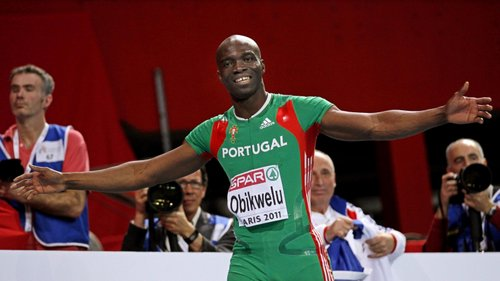
\includegraphics[scale=.35,angle=0]{francis.jpg}
            \caption{Francis Obikwelu}
            \label{fig:francis.2}
            \end{figure}
        \FloatBarrier
        
     \subsection{Atletas mundiais}
        \subsubsection{Usain Bolt}
        Usain St.Leo Bolt é um ex-velocista de origem jamaicana nascido a 21 de agosto de 1986. Este magnifico atleta possui vários recordes mundiais, os mais famosos dentro da pista são os dos 100m, 200m e da estafeta jamaicana de 4x100m (Nesta Carter, Michael Frater, Yohan Blake e Usain Bolt) onde esta equipa percorreu os quatro percursos em fantásticos 36.84s a 11 de agosto de 2012. Usain Bolt é dos atletas mais famosos fora e dentro do atletismo, não só pelas qualidades no atletismo mas também pela sua conectividade com os seus fãs. \cite{bolt}
         \FloatBarrier
            \begin{figure}[h]
            \center
            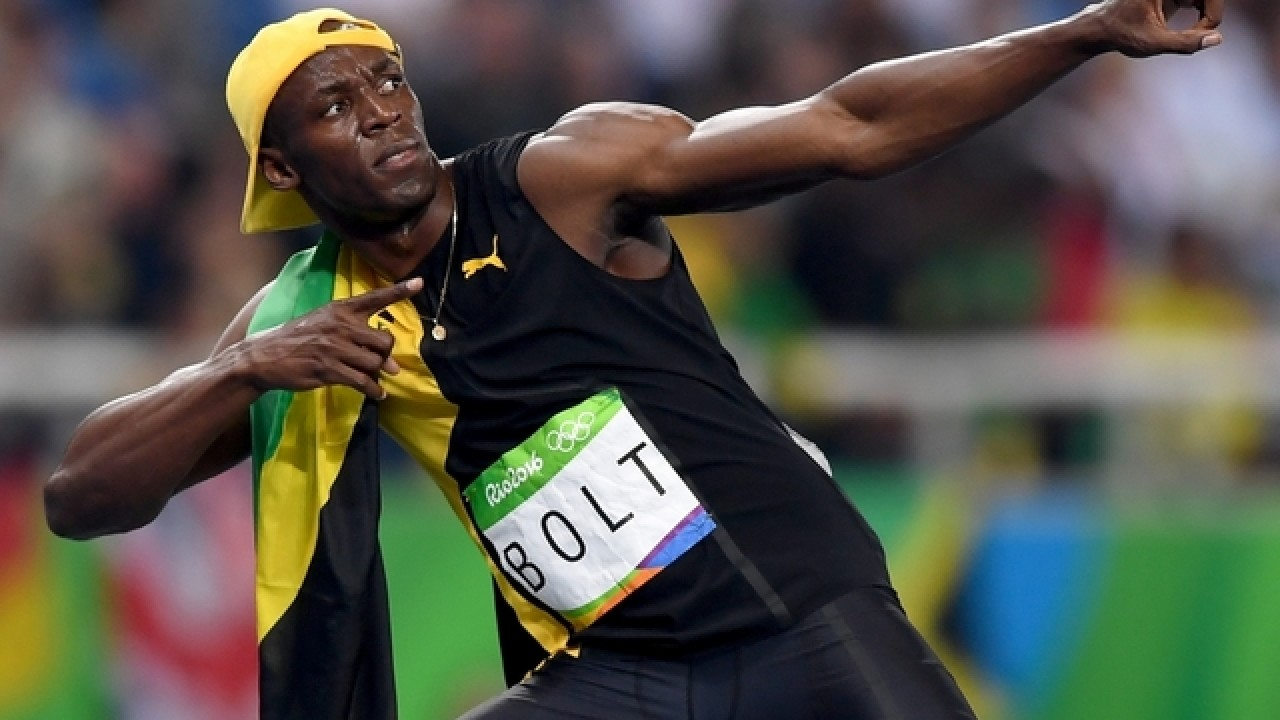
\includegraphics[scale=.14,angle=0]{bolt.jpg}
            \caption{Usain Bolt}
            \label{fig:Bolt.2}
            \end{figure}
        \FloatBarrier
        
        \subsubsection{Mo Farah}
        Mo Farah é um fundista britânico nascido a 23 de Março de 1983 que detêm todos os títulos possiveis. A especialidade deste atleta são os 5000m e 10000m. Este atleta é bicampeão olímpico de duas distâncias, sendo assim ele é tetracampeão olímpico, tem seis medalhas de ouro nas mesmas distâncias e três em campeonatos do mundo. Mo farah, nascido da Somália, foi eleito Atleta Europeu do Ano por dois anos consecutivos. \cite{mofarah}
        \FloatBarrier
            \begin{figure}[h]
            \center
            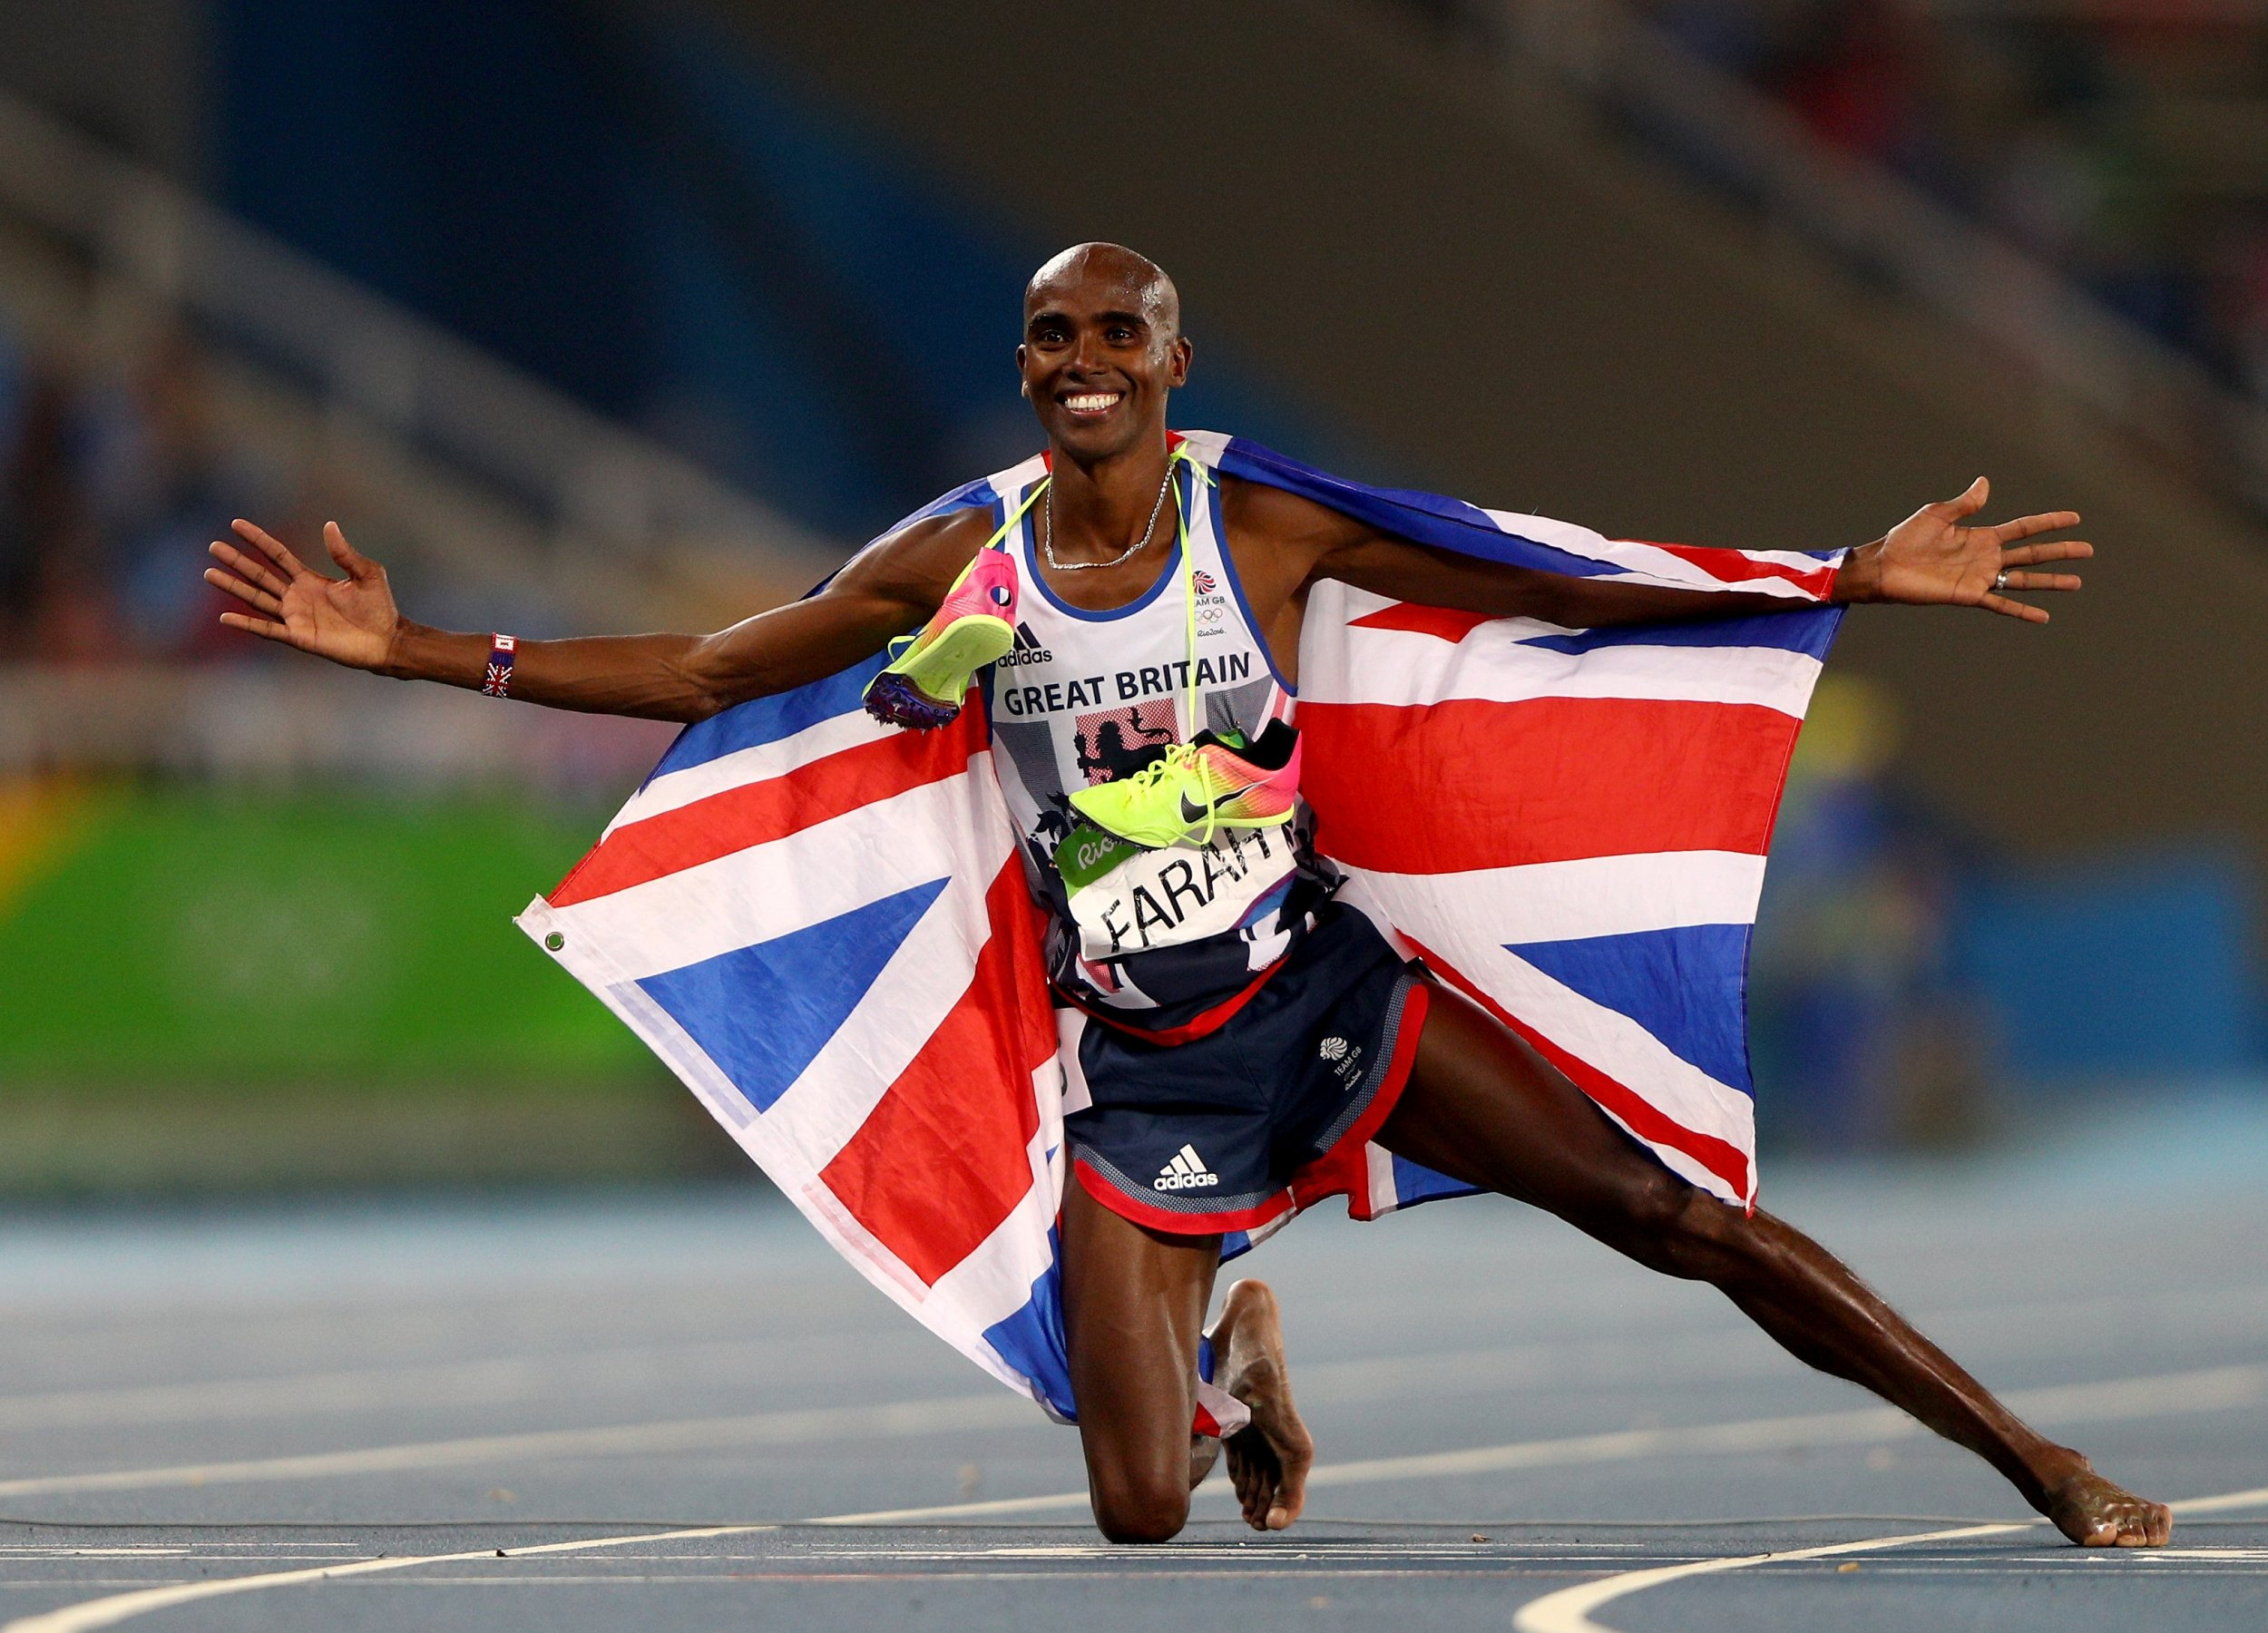
\includegraphics[scale=.09,angle=0]{mofarah.jpg}
            \caption{Mo Farah}
            \label{fig:Bolt.2}
            \end{figure}
        \FloatBarrier
        
        

\chapter{Conclusões}
\label{chap.Conclusões}
Correr, saltar e lançar é uma capacidade pré-adquirida desde a pré-história. Por esta modalidade passaram vários atletas e muitos deles deixaram uma grande marca na história do atletismo. \par
Como dizia o velocista Jamaicano, Usain Bolt “Sempre há limites. Eu não conheço os meus.”. Bolt conquistou oito medalhas de ouro na sua disciplina, velocidade, sendo dez vezes campeão mundial, de facto mostrou ao longo da sua carreira como atleta não conhecer os seus limites, dando sempre mais para conseguir atingir todos estes títulos. Também Carl Lewis, tem uma frase celebre – “Quero ser lembrado no futuro com alguém que inspirou outras pessoas a fazer coisas que pareciam impossíveis.”. Com estas frases os atletas pretendem inspirar futuros atletas a seguir sempre em frente perante as dificuldades pois ninguém sabe os seus limites, só há impossíveis quando deixamos de tentar, o que parece ser impossível deixa-o de ser quando alguém consegue alcançar esse tal impossível.\par
Terminamos este projeto frisando que o atletismo é uma modalidade bastante antiga e que faz parte da vida de muitos, diretamente ou indiretamente. Sendo assim é aconselhável a todos a prática de qualquer uma das disciplinas que fazem parte do atletismo, pois como vimos ao longo do trabalho são várias as vantagens que a prática do mesmo nos traz.   


\chapter*{Contribuições dos autores}

O trabalho foi dividido de forma igual tanto em termos de pesquisa como em termos de formulação do trabalho em \LaTeX. Tendo em conta que a maior parte do trabalho com exceção da pesquisa foi feito ao mesmo tempo na biblioteca.
A percentagem que deve ser atribuída a cada um dos autores é 50\% à \ac{AM}  e 50\% ao \ac{BL}.


%%%%%%%%%%%%%%%%%%%%%%%%%%%%%%%%%
\chapter*{Acrónimos}
\begin{acronym}
\acro{MIECT}[MIECT]{Mestrado Integrado em Engenharia de Computadores e Telemática}
\acro{AM}[AM]{Ana Monteiro}
\acro{BL}[BL]{Bruno Lemos}
\acro{UA}[UA]{Universidade de Aveiro}
\acro{DETI}[DETI]{Departamento de Electrónica, Telecomunicações e Informática}
\acro{GO}[GO]{Gordura e óleos}
\acro{LD}[LD]{Leite e derivados}
\acro{CPO}[CPO]{Carne, pescado e ovos}
\acro{Leg}[Leg]{Leguminosas}
\acro{CT}[CT]{Cereais e derivados, tubérculos}
\acro{Hort}[Hort]{Hortícolas}
\acro{Fru}[Frut]{Frutas}
\end{acronym}


%%%%%%%%%%%%%%%%%%%
\printbibliography



\end{document}
